\chapter{Thermodynamics}
\label{chap:thermo}

In this chapter, all of the theory related to the thermodynamics models
is presented.
The chapter begins with a review of fundamental concepts and relations
which are applicable for all gases in general.
These concepts and relations are stated without derivation;
texts on classical thermodynamics do a more authoritative job
with explanations and detailed derivations (see for example
Sonntag~et~al.~\cite{sonntag_etal_1998} or
\c{C}engel and Boles~\cite{cengel_boles_1998}).

The second section introduces the specific models
of gas behaviour that are implemented in the gas library.
The assumptions that apply to each of these models
are discussed and the equations defining the 
behaviour are presented.

\section{Fundamental concepts}

There are a number of thermodynamic properties which can be used
to quantify the state of a gas.
As we saw earlier, for CFD calculations we are interested in the
values of density, $\rho$, internal energy, $e$, pressure, $p$, 
and temperature, $T$.
Additionally, the sound speed, $a$, is a useful quantity when doing
the flux calculator computations.
Several other thermodynamic properties are used throughout the
gas library.
These are entropy, $s$, enthalpy, $h$, and the Gibbs function, $g$.
So, equations for these properties are also sought in the gas modelling.

The state of a pure gas (single species) is defined by two independent
properties.\footnote{In the case of gas mixtures, the species composition
is also required to uniquely specify the state of the gas.}
If the values of two independent properties are known, 
the other thermodynamic properties can be computed using the
equations of state for that gas.
An equation of state simply defines the relationship
between a set of thermodynamic properties.
It is convenient to distinguish equations of state
that link the pressure-volume-temperature relationship
(often called \textit{p-v-T} behaviour) from the equations of state
which characterise thermal behaviour, that is, how internal
energy varies with temperature and density.
The subsequent sections give more detail about the \textit{p-v-T} type
equations of state, and the thermal behaviour equations of state.
\footnote{The thermodynamics literature can sometimes cause some confusion
with regards to the phrase `equation of state'.
The literature will often refer to the \textit{p-v-T} behaviour of a gas as
its equation of state in the sense that it is the \emph{only}
equation of state that characterises the gas behaviour.
In other words, there is an implication that an equation of state is
nothing more (and nothing less) than a relation defining the \textit{p-v-T}
behaviour.
This is incorrect and ignores the fact that other properties of the gas
need to be linked via separate equations of state in order to completely
specify the gas behaviour.}
Given these two types of equation of state to model a specific gas
behaviour, the remainder of the properties can be computed from their
definitions or more fundamental relations.

\paragraph{A note on the symbol for internal energy}
In this report, internal energy is denoted with the symbol, $e$, whereas
many books on thermodynamics use the symbol, $u$.
The choice of $e$ is influenced by the use of the thermodynamics in the
context of fluid mechanics.
In fluid mechanics, the symbol $u$ is customarily used to represent
the flow speed in the $x$-direction.
It would rapidly become confusing to use the symbol $u$ to represent
internal energy also.
If comparing the equations here to other literature, the reader should bear
in mind that the symbol $e$ here will
often appear as $u$ in texts on thermodynamics.

\subsection{\textit{p-v-T} behaviour}
The equation of state which links the quantities of pressure, volume and temperature
is often referred to as the \textit{p-v-T} behaviour of a gas.
In the context of CFD, it is more convenient to use $\rho$ which is the
reciprocal of the specific volume, $v$.
So, for each of the gas models an equation of the form
\[ p = p(\rho, T) \]
is required.

As an example, consider a perfect gas: a gas where the collisions between particles are perfectly elastic
and the size of the particles is negligibly small compared
to the volume of their container.
For a perfect gas, the \textit{p-v-T} relation can be written as
\begin{equation}
   p = \rho R T
\end{equation}
where $R$ is the specific gas constant in units of J/(kg.K).
It may be computed from the universal gas constant and the molecular weight of the gas as $R = \frac{R_u}{M}$. 

As a second example, the van der Waal's equation of state for real gases is shown.
At high densities and low temperatures, the assumptions made for a perfect gas no longer hold.
We call this behaviour real gas behaviour.
One particular \textit{p-v-T} equation of state for real gases was written by van der Waal's
as
\begin{equation}
  \left ( p + a\rho^2 \right ) \left ( \frac{1}{\rho} - b \right ) = RT.
\end{equation}
In the above, the $a\rho^2$ term accounts for the intermolecular
forces particles exert on each other during collisions.
The $b$ term is called the co-volume.
It represents the finite volume occupied by the gas particles in
the container.
The constants $a$ and $b$ can be computed from a knowledge of
the critical point for a gas.
The expressions are
\begin{equation}
   a = \frac{27 R^2 T^2_{\text{cr}}}{64 P_{\text{cr}}}
\end{equation}
and
\begin{equation}
  b = \frac{R T_{\text{cr}}}{8 P_{\text{cr}}} \text{ . }
\end{equation}


\subsection{Thermal behaviour}
In addition to the \textit{p-v-T} behaviour of a gas, we
require expressions for the thermal behaviour of a gas in 
order to completely model the gas in a CFD context.
By thermal behaviour, we mean relationships for internal
energy in terms of other state variables (or equivalently,
relationships for enthalpy).
To form a general expression for internal energy,
we choose the starting point that internal energy
is a function of $T$ and $v$: $e = e(T,v)$.
After expansion with the chain rule and use of the
Maxwell relations,\footnote{
This is a standard derivation in most texts on classical thermodynamics.
See for example Section~10.4 of Sonntag~et~al.\ or Section~11-4 of
\c{C}engel and Boles.}
the general expression for a change
in energy from state 1 to state 2 is
\begin{equation}
 e_2 - e_1 = \int_{T_1}^{T_2} C_v dT +
             \int_{v_1}^{v_2} \left[ T\left(\frac{\partial p}{\partial T} \right)_v - p \right] dv \text{ . }
\label{eq:int-energy}
\end{equation}

As an example of an internal energy expression for a specific gas model,
consider again a perfect gas.
To our earlier assumptions about perfectly elastic collisions and
negligible co-volume, we add the restriction that the specific
heat at constant volume, $C_v$, is constant with temperature.
This is true for certain gases over a small temperature range.
It is valid for air at room temperature, for example.
Since $C_v$ is constant with temperature, the first integral
in Equation~\ref{eq:int-energy} becomes $C_v (T_2 - T_1)$.
Substituting the perfect gas relation, $p = \rho R T$,
into the second integral in Equation~\ref{eq:int-energy}
results in 0 for the second term.
For this `ideal' gas then, the expression for change in
internal energy is
\begin{equation}
  e_2 - e_1 = C_v (T_2 - T_1) \text{ . }
\end{equation}
It is common to see expressions for internal energy on its own, rather than
the \emph{change} in internal energy.
These expressions implicitly compute a change in energy: the change is
from a reference energy value.
In this case, let's arbitrarily set the energy $e_1$ to take
the value of 0 when the temperature $T_1$ is at 0 Kelvin.
Dropping the subscript '2' gives the familiar expression
for the internal energy of a calorically perfect gas
\begin{equation}
  e = C_v T \text{ . }
\end{equation}

In hypersonic flows, the assumption made above of constant specific heats is often violated.
Section~\ref{sec:gmodels} presents other models for the thermal behaviour
of a gas.

\subsection{Fundamental definitions and relations}
In this section, some fundamental definitions and relations of
thermodynamics are stated without derivation.
These are relations that are true for all gases regardless
of its particular behaviour.
We present these relations because they are used extensively
in the gas library to compute the various thermodynamic
properties.
Typically, the specific behaviour of a gas is established
by its \textit{p-v-T} behaviour and its thermal
behaviour.
The rest of its thermodynamic properties can then be computed
using the relations and definitions presented here.

Physically, enthalpy is the amount of heat that would be transferred
in a constant-pressure quasi-equilibrium process undergoing a change
in volume.
Enthalpy is defined in terms of internal energy, pressure and volume as
\begin{equation}
  h = e + pv \text{ . }
\end{equation}
The general expression for a change in entropy is
\begin{equation}
  \Delta s = \int_{T_1}^{T_2} \frac{C_p}{T}\,dT - \int_{p_1}^{p_2} \left ( \frac{\partial v}{\partial T} \right )_p\,dp \text{ . }
\end{equation}
An alternate expression for the change in entropy --- useful when the \textit{p-v-T}
equation of state is explicit in $p$ --- is
\begin{equation}
 \Delta s = \int_{T_1}^{T_2} \frac{C_v}{T}\,dT + \int_{v_1}^{v_2} \left( \frac{\partial p}{\partial T} \right)_v \, dv \text{ . }
\label{eq:s-p}
\end{equation}
The Gibbs function, $g$, is defined as
\begin{equation}
  g = h - Ts \text{ . }
\end{equation}

The specific heat at constant pressure is defined as
\begin{equation}
  C_p = \left ( \frac{\partial h}{\partial T} \right )_p \text{ , }
\end{equation}
and the definition of specific heat at constant volume is
\begin{equation}
  C_v = \left ( \frac{\partial e}{\partial T} \right )_v \text{ . }
\label{eq:Cv}
\end{equation}
The speed of sound in a gas is related to the pressure and density
by
\begin{equation}
  a^2 = \left ( \frac{\partial p}{\partial \rho} \right )_s \text{ . }
\end{equation}

The expressions presented here are useful for the most general of gas models.
For certain gas models, the general expressions may be simplified.
For example, the speed of sound in a perfect gas is $a = \sqrt{\gamma R T}$.
The gas library implements these simpler expressions when they are available,
otherwise the generalised expressions are used.

\section{Gas models}
\label{sec:gmodels}

In this section, the theory underlying the particular gas models available in the
gas library is presented.

\subsection{Classification of gases}
A user of the code may not be concerned with how the gas models are classified
internally in the code; the user is more interested just that there is a particular
gas model available to simulate the physical situation of interest.
However, in the interests of documenting the theory, this section discusses how
the various gas models are distinguished.
This classification is of interest to developer's of the library because
the theoretical classification is mirrored in the implementation.
The discussion presented here on gas classification follows that of
Anderson~\cite{anderson_1990}(see Section 10.1 of his text).

At the highest level, the models of gas behaviour are divided into
two classes based on their \textit{p-v-T} behaviour.
A gas model is classed as either:\\
\begin{tabular}{lp{12cm}}
\textbf{perfect:} & particle collisions are perfectly elastic;
                   the particles themselves occupy negligible volume (point particles); \emph{or} \\
\textbf{real:} & intermolecular forces exert some effect during particle collisions;
                the volume occupied by the particles themselves affects the calculation of gas behaviour.
\end{tabular}
At the pressures and temperatures typically encountered in aerodynamics, the assumption of perfect
gas behaviour is almost always valid.
It becomes important to model real gas behaviour at high densities and/or low temperatures.

\paragraph{Subclassification of perfect gases}
We noted earlier that when we use the perfect gas assumption in Equation~\ref{eq:int-energy}
for the internal energy of a gas, there is a functional dependence on temperature only.
\footnote{A derivation of this result is shown by \c{C}engel and Boles in
Example~11-8 of their text.}
We can further classify the group of perfect gases based on the form of this dependence on temperature.
These classifications are:\\
\begin{tabular}{lp{12cm}}
\textbf{calorically perfect:} & the specific heats $C_p$ and $C_v$ are constants; \emph{or} \\
\textbf{thermally perfect:} & the specific heats are variable and depend on temperature only.
\end{tabular}

The assumption of a calorically perfect gas is valid over a small temperature range and at moderate
temperatures (ie. room temperatures).
Over large temperature variations, particularly at higher temperatures, various internal energy modes
become increasingly more excited.
This leads to an observed variation in the specific heats with temperature, and consequently, 
a varying ratio of specific heats, $\gamma$.
This kind of behaviour is what is (or should be) referred to as high-temperature effects.

There is a third class of perfect gas considered in the gas library.
It is used to model gases which are not in thermal equilibrium.
We call these multi-temperature gases because the internal energy of the gas
is computed by ascribing different temperatures for different modes of the energy storage
(transitional, vibrational, etc.).
We defer discussion of this special class of gas to Section~\ref{sec:multi-T}.

\paragraph{Gas mixtures}
For mixtures of gases, the state of the gas depends on the mixture
composition and the properties of the individual components.
The properties of individual components have been considered
above when we classified gases as perfect or ideal.
What is needed then is a method for determining the mixture
properties based on the composition and properties of the components.
We can classify gas mixtures as\\
\begin{tabular}{lp{12cm}}
\textbf{perfect gas mixtures:} & each of the component gases exhibits perfect behaviour; \emph{or} \\
\textbf{real gas mixtures:} & each of the component gases exhibits perfect behaviour.
\end{tabular}

For perfect gas mixtures, the intensive mixture properties are simply a mass fraction weighted sum
of the component properties, while the extensive properties come from summing the individual contributions
of the components.
For real gas mixtures, the determination of mixture properties from component properties is more complex.
There are several methods available to calculate properties of real gas mixtures.
Those implemented in the gas library are discussed in Section~\ref{sec:real-gas-mix}.


\subsection{Calorically perfect gas (ideal gas)}
\label{sec:cal-perf}

\paragraph{Description}
The definition of a calorically perfect gas was introduced earlier as a gas with
constant specific heats.
Some literature refers to this kind of gas as an ideal gas.
In the gas library, the label \texttt{'ideal gas'} may be
used as a synonym to select a calorically perfect gas.
This model is fairly accurate over a small temperature range at moderate
temperatures.
For example, air at room temperature is modelled reasonably well as a pure substance
by taking $R = 287.1$\,J/(kg.K) and $\gamma = 1.4$.

\paragraph{Assumptions}
\begin{itemize}
\item The collisions between particles are perfectly elastic.
\item The particles are point particles; they occupy negligible volume per unit volume.
\item The specific heats $C_p$ and $C_v$ are constants.
\end{itemize}
Based on the last assumption, it follows that the ratio of specific heats, $\gamma$,
is also constant.

\paragraph{Equations}
The \textit{p-v-T} behaviour is simply the perfect gas equation of state:
\begin{equation}
 p = \rho R T \text{ . }
\end{equation}
The internal energy is computed as a function of temperature as
\begin{equation}
 e = C_v T + e_0
\end{equation}
where $e_0$ is the internal energy at a nominated reference state.
The value of specific entropy can be computed by referencing to
a standard state value $s_0$ at a temperature $T_0$ and pressure
$p_0$:
\begin{equation}
  s = C_p \log \frac{T}{T_0} - R \log \frac{p}{p_0} + s_0 \text{ . }
\end{equation}

\paragraph{Parameters}
The parameters of the model are described in Table~\ref{tab:cal-perfect-params}.
The table is divided between the required user inputs and derived parameters
which are computed based on the inputs.

\begin{table}[h]
\caption{Parameters for the calorically perfect gas model}
\label{tab:cal-perfect-params}
\begin{tabular}{llp{10cm}}
\toprule
Parameter & Units & Description \\ \midrule
\multicolumn{3}{l}{\textit{User input}} \\
$M$       & kg/mole & molecular weight of gas \\
$\gamma$  &  --    & ratio of specific heats, $C_p/C_v$ \\
$T_0$     & K      & temperature at the (user-chosen) standard state \\
$p_0$     & Pa     & pressure at the (user-chosen) standard state \\
$e_0$     & J/kg   & specific internal energy at (user-chosen) standard state.
                    When internal energy is computed, what is really 
                    reported is the \emph{change} in internal energy
                    from this reference or zero-point energy. \\
$s_0$     & J/(kg.K) & specific entropy at the (user-chosen) standard state.
                       As with internal energy, the computed entropy value
                       is the change from the standard state value of entropy. \\
 & & \\
\multicolumn{3}{l}{\textit{Derived parameters}} \\
$R$      & J/(kg.K) & specific gas constant computed as $R = R_u/M$ where
                      $R_u$ is the universal gas constant \\
$C_v$    & J/(kg.K) & specific heat at constant volume computed as \[C_v = R/(\gamma - 1)\] \\
$C_p$    & J/(kg.K) & specific heat at constant pressure computed as \[C_p = R + C_v\] \\
\bottomrule
\end{tabular}
\end{table}

\subsection{Thermally perfect gas}
\label{sec:therm-perf}
\paragraph{Description}
A thermally perfect gas is a gas in which $C_p$ and $C_v$ are functions of temperature
only.
Physically, this models a gas in which the internal energy modes are assumed to be
in thermal equilibrium at a single describing temperature.
This model for gas behaviour becomes important at higher temperatures as the 
internal energy modes of the particles are excited.
For example, the $C_p$ curve for diatomic oxygen is plotted in 
Figure~\ref{fig:Cp-O2}.

\begin{figure}[h]
\centering
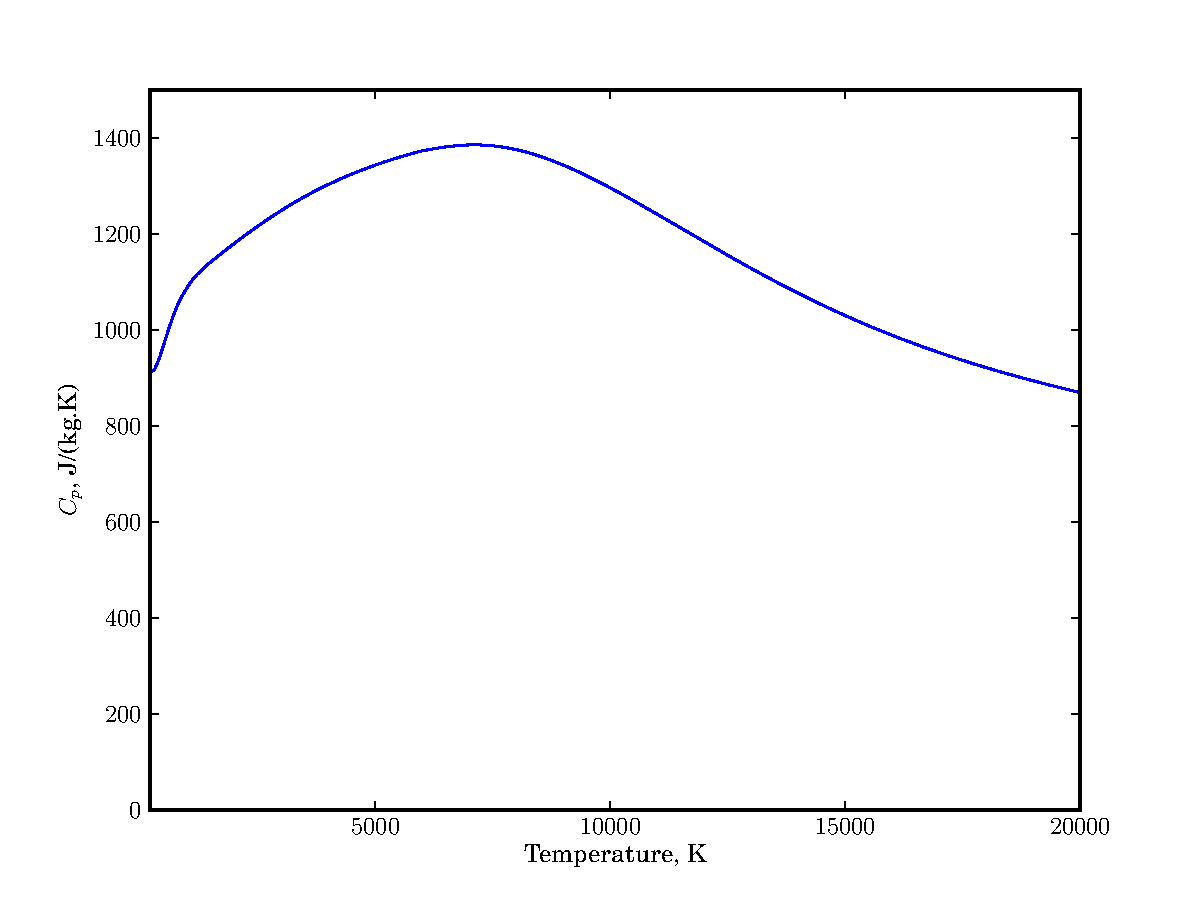
\includegraphics[width=12cm]{../figs/Cp-O2}
\caption[$C_p$ for diatomic oxygen]{Specific heat at constant pressure, $C_p$, for diatomic oxygen as a function of temperature.}
\label{fig:Cp-O2}
\end{figure}

\paragraph{Assumptions}
\begin{itemize}
\item The collisions between particles are perfectly elastic.
\item The particles are point particles; they occupy negligible volume per unit volume.
\item The specific heats $C_p$ and $C_v$ are functions of temperature only.
\end{itemize}
The last assumption implies that the gas is in thermal equilibrium.

\paragraph{Equations}
The \textit{p-v-T} behaviour is simply the perfect gas equation of state:
\begin{equation}
 p = \rho R T \text{ . }
\end{equation}
The internal energy is computed as a function of temperature as
\begin{equation}
 e(T) = \int_{T_0}^{T} C_v(T)\,dT + e_0
\end{equation}
where $e_0$ is the internal energy at a nominated reference state.
For some gases, a function for $C_p$ is available instead of $C_v$.
When that is the case, enthalpy may be evaluated as
\begin{equation}
\label{eq:tpg_h}
 h(T) = \int_{T_0}^{T} C_p(T)\,dT + h_0
\end{equation}
where $h_0$ in the specific enthalpy at a nominated reference state.
The internal energy is then computed from the definition of enthalpy
and applying the perfect gas equation of state:
\begin{equation}
 e = h - RT \text{ . }
\end{equation}

The value of specific entropy can be computed by referencing to
a standard state value $s_0$ at a temperature $T_0$ and pressure
$p_0$:
\begin{equation}
  s(p,T) = \int_{T_0}^{T} \frac{C_p(T)}{T}\,dT - R \log \frac{p}{p_0} + s_0 \text{ . }
\end{equation}

\paragraph{Input parameters}
The input parameters for the thermally perfect gas model
are given in Table~\ref{tab:tpg-params}.
A model for either $C_v$ or $C_p$ as a function
of temperature is required as an input.
Presently, the gas library implementation uses the 
CEA~\cite{mcbride_gordon_1996} polynomials for $C_p$
when modelling a thermally perfect gas.
The details of the CEA polynomials are presented in Appendix~\ref{sec:cea-thermo}.

\begin{table}[h]
\caption{Parameters for the thermally perfect gas model}
\label{tab:tpg-params}
\begin{tabular}{llp{10cm}}
\toprule
Parameter & Units & Description \\ \midrule
\multicolumn{3}{l}{\textit{User input}} \\
$M$       & kg/mole & molecular weight of gas \\
$\gamma$  &  --    & ratio of specific heats, $C_p/C_v$ \\
$T_0$     & K      & temperature at the (user-chosen) standard state \\
$p_0$     & Pa     & pressure at the (user-chosen) standard state \\
$e_0$     & J/kg   & specific internal energy at (user-chosen) standard state.
                    When internal energy is computed, what is really 
                    reported is the \emph{change} in internal energy
                    from this reference or zero-point energy. \\
$s_0$     & J/(kg.K) & specific entropy at the (user-chosen) standard state.
                       As with internal energy, the computed entropy value
                       is the change from the standard state value of entropy. \\
$C_v(T)$ \emph{or} $C_p(T)$ & J/(kg.K) & A model for $C_v$ or $C_p$ as a function of temperature only\\
 & & \\
\multicolumn{3}{l}{\textit{Derived parameter}} \\
$R$      & J/(kg.K) & specific gas constant computed as $R = R_u/M$ where
                      $R_u$ is the universal gas constant \\
\bottomrule
\end{tabular}
\end{table}

\subsection{Real gas}
\paragraph{Description}
At high densities and/or low temperatures, the behaviour of a gas is not well approximated by a perfect gas model.
We model this departure from perfect gas behaviour as a real gas.
The particular form of the \textit{p-v-T} relation varies depending the
model and assumptions that are applied.

\paragraph{Assumptions}
No assumptions about the behaviour of the gas are made.

\paragraph{Equations}
The \textit{p-v-T} relation for a real gas is particular to the
model which is used.
The subsequent sections detail the real gas models available
in the gas library.
In general form, we simply write
\begin{equation}
 p = p(\rho, T) \text{ . }
\end{equation}

The expression for internal energy is written in a general form
by referencing to an energy state, $e_0$, as
\begin{equation}
e = \int_{T_0}^{T} C_v\,dT + \int_{v_0}^{v} \left[ T\left(\frac{\partial p}{\partial T} \right)_v - p \right] dv \text{ . }
\label{eq:int-e-real}
\end{equation}
The evaluation of internal energy is split into two parts.
To compute the first term a model for $C_v$ is required, while the
second term can be computed from a knowledge of the \textit{p-v-T} 
behaviour.

\paragraph{Input parameters}
The ``real gas'' model does not describe any specific gas model,
rather it is generic label.
The specific real gas behaviour is set by selecting a model
for the \textit{p-v-T} behaviour and a model for $C_v$.
Thus Table~\ref{tab:real-gas} just lists the input parameters
in an abstract sense.

\begin{table}[h!]
\caption{Parameters for a real gas model}
\label{tab:real-gas}
\begin{tabular}{llp{10cm}}
\toprule
Parameter & Units & Description \\ \midrule
$M$       & kg/mole & molecular weight of gas \\
\textit{p-v-T} relation & & a model of the \textit{p-v-T} behaviour \\
$C_v$  & J/(kg.K) & a model for $C_v$ \\
\bottomrule
\end{tabular}
\end{table}

\paragraph{Various models of real gas \textit{p-v-T} behaviour}
The following lists the various types of real gases that are modelled
by the gas library.
The details of these models are presented in the subsequent sections.
This list of available real gases is:
\begin{itemize}
\item van der Waal's gas (Section~\ref{sec:van_der_waals_gas})
\item Noble-Abel gas (Section~\ref{sec:noble_abel_gas})
\item Bender gas (Section~\ref{sec:bender_gas})
\item Modified Benedict-Webb-Rubin (MBWR) gas (Section~\ref{sec:MBWR_gas})
\item REFPROP gas (Section~\ref{sec:REFPROP_gas})
\end{itemize}

\subsection{van der Waal's gas}
\label{sec:van_der_waals_gas}
\paragraph{Description}
Van der Waal's proposed a modification to the perfect
gas equation of state to account for the intermolecular
forces between particles during collisions and
the finite volume occupied by the particles.

\paragraph{Equations}
The van der Waal's \textit{p-v-T} relation can be written
in terms of density, $\rho$, as
\begin{equation}
  \left ( p + a\rho^2 \right ) \left ( \frac{1}{\rho} - b \right ) = RT \text{ . }
\end{equation}
Substituting this equation in terms of $p$ and $T$ into Equation~\ref{eq:int-e-real} for the internal energy of a real gas, the second term may be integrated to yield an expression for internal energy:
\begin{equation}
e(T, \rho) = \int_{T_0}^{T} C_v\,dT + a \left( \rho - \rho_0 \right) \text{ . }
\end{equation}
Note that this relation still depends on some choice for modelling $C_v$.
Similarly, the second term in the expression for entropy (Equation~\ref{eq:s-p})
may be evaluated analytically, while the first term depends on the model for $C_v$:
\begin{equation}
s(T,p) = \int_{T_0}^{T} \frac{C_v}{T}\,dT + \left [ R \log \left( v - b \right ) \right ]_{v_0}^{v} \text { . }
\end{equation}


The constants $a$ and $b$ are computed from the critical point pressure and
temperature for the gas.
\begin{equation}
   a = \frac{27 R^2 T^2_{\text{cr}}}{64 P_{\text{cr}}} \qquad \text{and} \qquad
   b = \frac{R T_{\text{cr}}}{8 P_{\text{cr}}}
\end{equation}
Here $b$ is the co-volume of the gas, sometimes written as $\nu_0$.
In the expression above for internal energy, $\rho_0 = \frac{1}{\nu_0}$.

\paragraph{Input parameters}

\begin{table}[h!]
\caption{Parameters for the van der Waal's gas model}
\label{tab:vdw-params}
\begin{tabular}{llp{10cm}}
\toprule
Parameter & Units & Description \\ \midrule
\multicolumn{3}{l}{\textit{User input}} \\
$M$       & kg/mole & molecular weight of gas \\
$T_0$     & K      & temperature at the (user-chosen) standard state \\
$p_0$     & Pa     & pressure at the (user-chosen) standard state \\
$e_0$     & J/kg   & specific internal energy at (user-chosen) standard state.
                    When internal energy is computed, what is really 
                    reported is the \emph{change} in internal energy
                    from this reference or zero-point energy. \\
$s_0$     & J/(kg.K) & specific entropy at the (user-chosen) standard state.
                       As with internal energy, the computed entropy value
                       is the change from the standard state value of entropy. \\
$p_c$     & Pa     & critical point pressure \\
$T_c$     & K      & critical point temperature \\
 & & \\
\multicolumn{3}{l}{\textit{Derived parameters}} \\
$R$      & J/(kg.K) & specific gas constant computed as $R = R_u/M$ where
                      $R_u$ is the universal gas constant \\
$a$      & J$^2$/(kg$^2$Pa) & constant accounting for the effect of intermolecular forces
                              computed as \[ a = \frac{27 R^2 T^2_{\text{cr}}}{64 P_{\text{cr}}} \] \\
$b$      & m$^3$/kg & co-volume (sometimes seen as $\nu_0$) computed as
                      \[ b = \frac{R T_{\text{cr}}}{8 P_{\text{cr}}} \] \\

\bottomrule
\end{tabular}
\end{table}

\subsection{Noble-Abel gas}
\label{sec:noble_abel_gas}
\paragraph{Description}
The Noble-Abel gas model for real gas behaviour is a simplification of
the van der Waal's model in that it only accounts for the co-volume
occupied by the gas particles.
This model is applicable at high pressures where the volume of
the particles is an appreciable fraction of the total occupied volume
but the collision interactions are not significantly affected
by intermolecular forces.
This may be the case at high temperatures where the collisions
occur relatively quickly, not allowing much time for the intermolecular
forces to exert an effect.
The Noble-Abel gas model is frequently used when simulating interior
ballistics.

\paragraph{Equations}
The \textit{p-v-T} behaviour for a Noble-Abel gas is expressed as
\begin{equation}
  p \left( \frac{1}{\rho} - b \right ) = RT \text{ . }
\end{equation}

Since $\left( \frac{\partial p}{\partial T} \right)_v$ evaluates to the same analytical expression as in the case of a van der Waal's case, the expressions for internal
energy and entropy are the same:
\begin{equation}
e(T, \rho) = \int_{T_0}^{T} C_v\,dT + a \left( \rho - \rho_0 \right) \text{ , }
\end{equation}
and 
\begin{equation}
s(T,p) = \int_{T_0}^{T} \frac{C_v}{T}\,dT + \left [ R \log \left( v - b \right ) \right ]_{v_0}^{v} \text { . }
\end{equation}

Again, the co-volume $b$ is computed as
\begin{equation}
   b = \frac{R T_{\text{cr}}}{8 P_{\text{cr}}} \text{ . }
\end{equation}
Note, sometimes $b$ is specified directly for certain gases.
It may be more accurate to use an empirically-derived value
over a certain pressure and temperature range.

\paragraph{Input parameters}

\begin{table}[h]
\caption{Parameters for the Noble-Abel gas model}
\label{tab:na-params}
\begin{tabular}{llp{10cm}}
\toprule
Parameter & Units & Description \\ \midrule
\multicolumn{3}{l}{\textit{User input}} \\
$M$       & kg/mole & molecular weight of gas \\
$T_0$     & K      & temperature at the (user-chosen) standard state \\
$p_0$     & Pa     & pressure at the (user-chosen) standard state \\
$e_0$     & J/kg   & specific internal energy at (user-chosen) standard state.
                    When internal energy is computed, what is really 
                    reported is the \emph{change} in internal energy
                    from this reference or zero-point energy. \\
$s_0$     & J/(kg.K) & specific entropy at the (user-chosen) standard state.
                       As with internal energy, the computed entropy value
                       is the change from the standard state value of entropy. \\
$p_c$     & Pa     & critical point pressure \\
$T_c$     & K      & critical point temperature \\
 & & \\
\multicolumn{3}{l}{\textit{Derived parameters}} \\
$R$      & J/(kg.K) & specific gas constant computed as $R = R_u/M$ where
                      $R_u$ is the universal gas constant \\
$b$      & m$^3$/kg & co-volume (sometimes seen as $\nu_0$) computed as
                      \[ b = \frac{R T_{\text{cr}}}{8 P_{\text{cr}}} \] \\

\bottomrule
\end{tabular}
\end{table}

\subsection{Bender gas}
\label{sec:bender_gas}

\paragraph{Description}
The Bender gas model for real gas behaviour uses the Bender \cite{bender1975equations}
\textit{p-v-T} relationship which is a modification of the Benedict-Webb-Rubin
form \cite{sengers2000equations}.
The Bender \textit{p-v-T} relationship has 19 experimentally determined coefficients
which have been published for over 50 substances \cite{bender1970equations}
\cite{bender1975equations} \cite{platzer1990thermophysical} \cite{polt1992bender}
\cite{sievers1980equation}.

This model is applicable at high pressures and densities, in the critical region and
for calculating vapour-liquid equilibrium. For this reason, it is useful in
simulating flows which are thermodynamically close to or within the vapour dome,
such as turbomachinery and nozzle flows.

%\paragraph{Assumptions}
\paragraph{Equations}
The \textit{p-v-T} behaviour for a Bender gas is expressed by the Bender equation of state \cite{bender1975equations}
\begin{dmath}
P = \rho R T + \rho^2 \sum_{i=1}^5 A_i T^{2-i} + \rho^3 \sum_{i=6}^8 A_i T^{7-i}
    + \rho^4 \left( A_9 T + A_{10} \right) + \rho^5 \left( A_{11} T + A_{12} \right) + \rho^6 A_{13}
    + \left[ \rho^3 \sum_{i=14}^{16} A_i T^{12-i} + \rho^5 \sum_{i=17}^{19} A_i T^{15-i} \right] \exp(-A_{20} \rho^2)
\end{dmath}
Where \(A_i\) are the experimentally determined coefficients. To capture the
\textit{p-v-T} behaviour in the critical region, the final coefficient is typically
published as
\begin{dmath}
A_{20} \approx \rho_c^{-2}
\end{dmath}
The ideal gas (zero density) specific heat capacity at constant pressure is
expressed using a fourth order polynomial, as this form can be used with
the available published coefficients \cite{platzer1990thermophysical}
\cite{polt1992bender} \cite{mclinden1989measurement}
\cite{huber1992thermodynamic} \cite{outcalt1995equations}
\cite{outcalt1996modified} \cite{outcalt1997equation}
\cite{reynolds1979thermodynamic}
\begin{dmath} \label{eq:bender_cp0}
C_p^0 = \sum_{i=1}^6 G_i T^{i-2}
\end{dmath}

Reynolds \cite{reynolds1979thermodynamic} provide coefficients for a \(C_v^0\) equation,
which have been converted to \(C_p^0\) form using
\begin{dmath}
C_p^0 = C_v^0 + R
\end{dmath}
which results in only one coefficient modification
\begin{dmath}
G_{2,p} = G_{2,v} + R
\end{dmath}

Due to the polynomial and exponential form of the Bender \textit{p-v-T} relationship
and the ideal gas specific heat capacity equation,
the expressions for internal energy, entropy, real specific heat capacities and
sound speed can be evaluated analytically.

For the calculation of internal energy, Equation~\ref{eq:int-energy} can be
re-written as \cite{reynolds1979thermodynamic}
\begin{dmath}
e = \int_{T_0}^T \left(C_p^0 - R\right)\, dT
    + \int_0^{\rho}\frac{1}{\rho^2}\left[ P - T\left( \frac{\partial P}{\partial T} \right)_{\rho} \right]\, d\rho
    + e_0
\end{dmath}
For the calculation of entropy, Equation~\ref{eq:s-p} can be
re-written as \cite{reynolds1979thermodynamic}
\begin{dmath}
s = \int_{T_0}^T \frac{C_p^0 - R}{T}\, dT
    - R \ln{\rho}
    + \int_0^{\rho}\frac{1}{\rho^2}\left[ \rho R - \left( \frac{\partial P}{\partial T} \right)_{\rho} \right]\, d\rho
    + s_0
\end{dmath}
\(C_v\) can then be calculated analytically with Equation~\ref{eq:Cv}. \(C_p\) is
calculated using the Mayer Relation and the chain rule
\begin{dmath}
C_p = C_v + T\left(\frac{\partial\nu}{\partial T}\right)_P\left(\frac{\partial P}{\partial T}\right)_{\nu}
= C_v - T \rho^{-2} \left(\frac{\partial\rho}{\partial T}\right)_P\left(\frac{\partial P}{\partial T}\right)_{\rho}
\end{dmath}
The sound speed is given by
\begin{dmath}
a = \sqrt{\frac{C_p}{C_v} \left(\frac{\partial P}{\partial \rho}\right)_T}
\end{dmath}
The analytical derivation using the above equations can be performed by hand, but
is quite verbose and has therefore not been included in this report.

\paragraph{Input parameters}
The input parameters for the Bender gas model are given in Table~\ref{tab:bender-params}.

\begin{table}[h]
\caption{Parameters for the Bender gas model}
\label{tab:bender-params}
\begin{tabular}{llp{10cm}}
\toprule
Parameter & Units & Description \\ \midrule
\multicolumn{3}{l}{\textit{User input}} \\
$M$       & kg/mole & molecular weight of gas \\
$A_i$     &       & \textit{p-v-T} equation coefficients \\
$G_i$     &       & ideal gas specific heat capacity equation coefficients \\
$T_0$     & K     & temperature at the standard reference state \\
$e_0$     & J/kg   & specific internal energy at the standard reference state.
                    When internal energy is computed, what is really 
                    reported is the \emph{change} in internal energy
                    from this reference or zero-point energy. \\
$s_0$     & J/(kg.K) & specific entropy at the standard reference state.
                       As with internal energy, the computed entropy value
                       is the change from the standard state value of entropy. \\
 & & \\
\multicolumn{3}{l}{\textit{Derived parameters}} \\
$R$      & J/(kg.K) & specific gas constant computed as $R = R_u/M$ where
                      $R_u$ is the universal gas constant \\
\bottomrule
\end{tabular}
\end{table}

\subsection{MBWR gas}
\label{sec:MBWR_gas}

\paragraph{Description}
The MBWR gas model for real gas behaviour uses the Jacobsen and Stewart
\cite{jacobsen1973thermodynamic} \textit{p-v-T} relationship, which became known
as the Modified Benedict-Webb-Rubin (MBWR) equation \cite{span2000multiparameter}.
The MBWR \textit{p-v-T} relationship has 32 experimentally determined coefficients,
and has been used extensively in technical and scientific applications \cite{sengers2000equations}.

This model is applicable at high pressures and densities, in the critical region and
for calculating vapour-liquid equilibrium. For this reason, it is useful in
simulating flows which are thermodynamically close to or within the vapour dome,
such as turbomachinery and nozzle flows. The higher number of coefficients in
comparison to the Bender \textit{p-v-T} relationship mean that the MBWR equation
typically has higher accuracy in the evaluation of thermodynamic properties.

%\paragraph{Assumptions}
\paragraph{Equations}
The \textit{p-v-T} behaviour for a MBWR gas is expressed by the MBWR equation of state \cite{jacobsen1973thermodynamic}
\begin{dmath}
P = \sum_{i=1}^9 A_i \rho^i + \exp{\left(-\gamma \rho^2\right)}\sum_{i=10}^{15} A_i \rho^{2i-17}
\end{dmath}
where the critical region coefficient is
\begin{dmath}
\gamma = \rho_c^{-2}
\end{dmath}
and the \(A_i\) temperature polynomials are
\begin{align*}
A_1 &= RT\\
A_2 &= B_1 T + B_2 T^{0.5} + B_3 + B_4 T^{-1} + B_5 T^{-2}\\
A_3 &= B_6 T + B_7 + B_8 T^{-1} + B_9 T^{-2}\\
A_4 &= B_{10} T + B_{11} + B_{12} T^{-1}\\
A_5 &= B_{13}\\
A_6 &= B_{14} T^{-1} + B_{15} T^{-2}\\
A_7 &= B_{16} T^{-1}\\
A_8 &= B_{17} T^{-1} + B_{18} T^{-2}\\
A_9 &= B_{19} T^{-2}\\
A_{10} &= B_{20} T^{-2} + B_{21} T^{-3}\\
A_{11} &= B_{22} T^{-2} + B_{23} T^{-4}\\
A_{12} &= B_{24} T^{-2} + B_{25} T^{-3}\\
A_{13} &= B_{26} T^{-2} + B_{27} T^{-4}\\
A_{14} &= B_{28} T^{-2} + B_{29} T^{-3}\\
A_{15} &= B_{30} T^{-2} + B_{31} T^{-3} + B_{32} T^{-4}\\
\end{align*}
The ideal gas (zero density) specific heat capacity at constant pressure is
expressed using Equation~\ref{eq:bender_cp0}, and the internal energy, entropy,
real specific heat capacities and sound speed can be evaluated analytically with
the same approach as used in Section~\ref{sec:bender_gas}. The analytical
derivation using these equations can be performed by hand, but are quite verbose
and has therefore not been included in this report.

\paragraph{Input parameters}
The input parameters for the MBWR gas model are given in Table~\ref{tab:MBWR-params}.

\begin{table}[h]
\caption{Parameters for the MBWR gas model}
\label{tab:MBWR-params}
\begin{tabular}{llp{10cm}}
\toprule
Parameter & Units & Description \\ \midrule
\multicolumn{3}{l}{\textit{User input}} \\
$M$       & kg/mole & molecular weight of gas \\
$B_i$     &       & \textit{p-v-T} equation coefficients \\
$G_i$     &       & ideal gas specific heat capacity equation coefficients \\
$T_0$     & K     & temperature at the standard reference state \\
$e_0$     & J/kg   & specific internal energy at the standard reference state.
                    When internal energy is computed, what is really 
                    reported is the \emph{change} in internal energy
                    from this reference or zero-point energy. \\
$s_0$     & J/(kg.K) & specific entropy at the standard reference state.
                       As with internal energy, the computed entropy value
                       is the change from the standard state value of entropy. \\
 & & \\
\multicolumn{3}{l}{\textit{Derived parameters}} \\
$R$      & J/(kg.K) & specific gas constant computed as $R = R_u/M$ where
                      $R_u$ is the universal gas constant \\
\bottomrule
\end{tabular}
\end{table}

\subsection{REFPROP gas}
\label{sec:REFPROP_gas}

\paragraph{Description}
The REFPROP gas model for real gas behaviour makes use of the NIST REFPROP
thermodynamic and transport property database (Version 9) \cite{lemmon2002nist}
for the evaluation of all fluid properties. REFPROP is a commercial software package
that implements the most accurate models and equations available for the
evaluation of pure fluid and mixture properties. Typically, thermodynamic and transport
properties can be evaluated to within the uncertainly of the experimental data with
which the equations are based.

This model is applicable at high pressures and densities, in the critical region and
for calculating vapour-liquid equilibrium. For this reason, it is useful in
simulating flows which are thermodynamically close to or within the vapour dome,
such as turbomachinery and nozzle flows. The equations used in REFPROP are
more accurate than the equations used in the MBWR gas model, and also cover
many fluid mixtures.

%\paragraph{Assumptions}
\paragraph{Equations}
The REFPROP database makes use of optimized multiparameter fundamental equations
of state, known as the Helmholtz equation of state. For a comprehensive description of
the Helmholtz equation of state and its use, refer to the text of Span \cite{span2000multiparameter}.

\paragraph{Input parameters}
All required inputs for the REFPROP gas model are covered by the REFPROP software,
which contains fluid and mixture specific configuration files.

\subsection{Perfect gas mixtures}
\label{sec:pgm}
\paragraph{Description}
A perfect gas mixture, as the name implies, is a gas composed
of individual components each having perfect gas behaviour.
This model is typically used when simulating chemically
reacting gases; each chemical species is treated as a separate
component of the gas mixture.
Usually, it makes physical sense to assume that each of the component species
has the same thermal behaviour.
This leads to the special cases of calorically perfect gas mixtures and
thermally perfect gas mixtures.
The equations describing the mixture properties are the same in both
instances. 

\paragraph{Assumptions}
\begin{itemize}
\item Each component of the gas exhibits perfect behaviour.
\item The Gibbs-Dalton law holds: the properties of individual
      component gases are not influenced by the presence of
      other gases, and each component in the mixture behaves
      as if it existed alone at mixture temperature and volume.
\end{itemize}

\paragraph{Equations}
For mixtures, the thermodynamic state is uniquely defined
by specifying two independent properties of the mixture and the mixture
composition.
The subscript $m$ is used to denote mixture properties.
By applying Dalton's Law of partial pressures, the
\textit{p-v-T} behaviour for a mixture of perfect
gases is
\begin{equation}
 p_m = \sum_{i=1}^N \rho_i R_i T \text{ . }
\end{equation}
The internal energy for the mixture, $e_m$, is computed as
a mass fraction weighted sum of the component
internal energies
\begin{equation}
 e_m = \sum_{i=1}^N f_i e_i(T_m) \text{ . }
\end{equation}
A number of other mixture properties are also computed
as a mass fraction weighted sum.
The entropy of the mixture is
\begin{equation}
 s_m = \sum_{i=1}^N f_i s_i(T_m, p_m) \text{ . }
\end{equation}
The specific gas constant of the mixture is
\begin{equation}
 R_m = \sum_{i=1}^N f_i R_i \text{ . }
\end{equation}
The specific heats are
\begin{equation}
  C_{p_m} = \sum_{i=1}^N f_i C_{p_i} \text{ , }
\end{equation}
and
\begin{equation}
  C_{v_m} = \sum_{i=1}^N f_i C_{v_i} \text{ . }
\end{equation}
The mixture molecular weight is computed as a mole fraction
weighted sum as
\begin{equation}
  M_m = \sum_{i=1}^N y_i M_i \text{ . }
\end{equation}

\paragraph{Input parameters}
The input for the model is a list of the component gaseous species.
For each species, a specific perfect gas model needs to be selected
(and appropriate inputs given).
The available gas models for the components is a selection of a calorically perfect
gas (Section~\ref{sec:cal-perf}) or thermally perfect gas (Section~\ref{sec:therm-perf}).

\subsection{Real gas mixtures}
\label{sec:real-gas-mix}
\paragraph{Description}
The model of real gas mixtures assumes that all of the
component gases have real gas behaviour.
This model is useful for interior ballistics simulations
where there are a number of component gases such
as air and propellant combustion products.

\paragraph{Assumptions}
The properties for a mixture of real gases are more complex to compute
than those for a mixture of real gases.
Dalton's Law of Partial Pressures and Amagat's Law of Additive Volumes
do not hold exactly but can be applied to give an approximate
treatment.
An alternative approach, and the one used in the gas library,
is to assume the gas mixture behaves as a pseudopure substance.

\paragraph{Equations}
The \textit{p-v-T} behaviour of the gas is computed by assuming
either van der Waal's behaviour
\begin{equation}
  \left ( p_m + a_m\rho_m^2 \right ) \left ( \frac{1}{\rho_m} - b_m \right ) = R_mT_m \text{ , }
\end{equation}
or Noble-Abel behaviour
\begin{equation}
  p_m \left( \frac{1}{\rho_m} - b_m \right ) = R_mT_m \text{ . }
\end{equation}
The mixture constants $a_m$ and $b_m$ are computed as
\begin{equation}
  a_m = \left( \sum_{i=1}^N y_i \sqrt{a_i} \right)^2 \qquad \text{and} \qquad 
  b_m = \sum_{i=1}^N y_i b_i \text{ . }
\end{equation}
The mixture gas constant is as 
\begin{equation}
R_m = \sum_{i=1}^N f_i R_i \text{ . }
\end{equation}
The remainder of the mixture properties are computed in
the same manner as for the mixture of perfect gases (see Section~\ref{sec:pgm}).


\paragraph{Input parameters}
The input for the model is a list of the component gaseous species and
the type of real gas model (either van der Waal's or Noble-Abel).
For each species, the parameters for the specific real gas model need to be set.

\subsection{Multi-temperature gas mixtures}
\label{sec:multi-T}
\paragraph{Description}
\paragraph{Assumptions}
\paragraph{Equations}
\paragraph{Input parameters}


